\documentclass{TIJMUjiaoanLL}
\pagestyle{empty}

\begin{document}

\kecheng{分子生物计算}
\neirong{编程的艺术 \ / 第3章}
\jiaoshi{伊现富}
\zhicheng{讲师}
\riqi{2016年11月16日13:30-15:30}
\duixiang{生物医学工程与技术学院2013级生信班(本)}
\renshu{30}
\fangshi{理论讲授}
\xueshi{2}
\jiaocai{Perl语言在生物信息学中的应用——基础篇}

\firstHeader
\maketitle
\thispagestyle{empty}

\mudi{
\begin{itemize}
  \item 掌握:编程的策略、步骤和基本流程;调试程序的主要方法。
  \item 熟悉:学习编程的主要方法;伪代码的编写与解读。
  \item 了解:Git在版本控制中的应用。
  \item 自学:GitHub的使用。
\end{itemize}
}

\fenpei{
\begin{itemize}
  \item (5')引言与导入:回顾学习C语言和Linux的经历。
  \item (10')学习方法:总结学习编程的各种方法。
  \item (35')编程流程:介绍编程的基本流程,介绍版本控制的概念,详细讲解Git的使用。
  \item (10')编程策略:总结编程的主要策略。
  \item (35')编程过程:通过实例讲解编程的基本步骤,介绍伪代码和代码注释。
  \item (5')总结与答疑:总结授课内容中的知识点与技能,解答学生疑问。
\end{itemize}
}

\zhongdian{
\begin{itemize}
  \item 重点:编程的策略、步骤和流程。
  \item 难点:编程的步骤和流程。
  \item 解决策略:通过实例演示帮助学生理解、记忆。
\end{itemize}
}

\waiyu{
\vspace*{-10pt}
\begin{multicols}{2}
版本控制系统(VCS,Version Control System)

算法(algorithm)

伪代码(pseudocode)

注释(comment)
\end{multicols}
\vspace*{-10pt}
}

\fuzhu{
\begin{itemize}
  \item 多媒体:编程中的版本控制;伪代码。
  \item 板书:编程的基本流程;解释算法的实例。
  \item 演示:Git的使用。
\end{itemize}
}

\sikao{
\vspace*{-10pt}
\begin{multicols}{2}
\begin{itemize}
  \item 总结学习编程语言的主要方法。
  \item 编写程序的基本流程是什么?
  \item 如何使用Git进行版本控制。
  \item 总结调试程序的方法。
  \item 总结常用的编程策略。
  \item 编程的基本过程是怎么样的?
  \item 在编程过程中需要构思哪些内容?
  \item 使用伪代码和注释有哪些优势?
\end{itemize}
\end{multicols}
\vspace*{-10pt}
}

\cankao{
\begin{itemize}
  \item Beginning Perl for Bioinformatics, James Tisdall, O'Reilly Media, 2001.
  \item Perl语言入门(第六版),Randal L. Schwartz, brian d foy \& Tom Phoenix著,盛春\ 译,东南大学出版社,2012。
  \item Mastering Perl for Bioinformatics, James Tisdall, O'Reilly Media, 2003.
  \item 维基百科等网络资源。
\end{itemize}
}

\firstTail

\newpage
\otherHeader

\begin{enumerate}
  \item 引言与导入(5分钟)\textcolor{red}{(引导学生进行回顾)}
    \begin{itemize}
      \item C语言的学习:听课、编程、练习……
      \item Linux系统的学习:听课、自学、练习……
    \end{itemize}
  \item 学习方法(10分钟)\textcolor{red}{(通过自己的亲身经历进行讲解)}
    \begin{enumerate}
      \item 最佳方法:适合自己的才是最好的!(取决于任务属性、时间限制、个人喜好……)
      \item 常见方法:参加培训班、阅读书籍、死啃手册、拜师学艺、研读程序……
      \item 五字真言:实践出真知!(Experience is the best teacher.)
    \end{enumerate}
  \item \textcolor{red}{【重点、难点】}编程流程(35分钟)\textcolor{red}{(通过实例进行讲解)}
    \begin{enumerate}
      \item 基本流程:编辑-运行-修正
      \item 版本控制
	\begin{enumerate}
	  \item 简介:一种记录若干文件内容变化,以便将来查阅特定版本修订情况的系统
	  \item Git
	    \begin{itemize}
	      \item 简介:分散式版本控制软件,Linus Torvalds,2005年
	      \item 使用\textcolor{red}{(通过简单的实例演示使用方法)}
	    \end{itemize}
	  \item GitHub:一个共享虚拟主机服务,用于存放使用Git版本控制的软件代码和内容项目;世界上最大的代码存放网站
	\end{enumerate}
\vspace*{-1em}
\begin{multicols}{2}
      \item 错误信息
	\begin{itemize}
	  \item 出现错误并不可怕
	  \item 一定不要视而不见
	  \item 从第一个错误开始修复
	  \item 必要时进行一定的猜测
	\end{itemize}
      \item 调试程序
	\begin{itemize}
	  \item Perl调试器:\verb|perl -d script.pl|
	  \item 加入print语句
	  \item 选择性得注释掉部分代码
	  \item 模块:Benchmark, Data::Dumper, Smart::Comments, ...
	\end{itemize}
\end{multicols}
\vspace*{-1em}
\begin{figure}[h]
  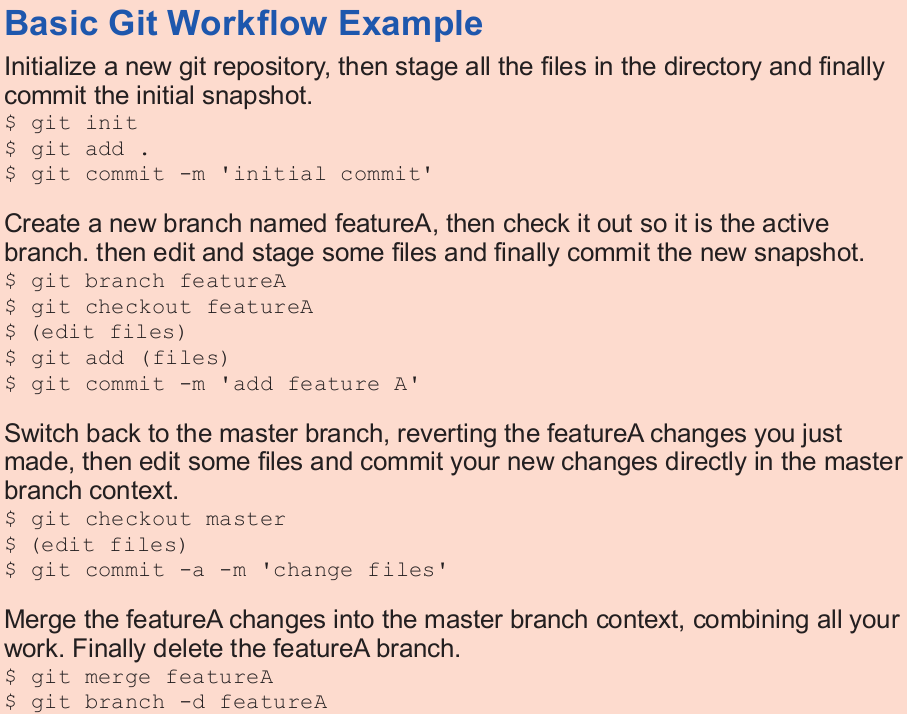
\includegraphics[width=0.5\textwidth]{c3.programming.git.png}
  \includegraphics[width=0.55\textwidth]{c3.programming.github.png}
\end{figure}
    \end{enumerate}
  \item \textcolor{red}{【重点】}编程策略(10分钟)\textcolor{red}{(通过现实中的例子进行讲解)}
    \begin{enumerate}
      \item 寻找现成的程序\textcolor{red}{(避免重复发明轮子)}
      \item 自己编写程序
	\begin{enumerate}
	  \item 修改现成的程序\textcolor{red}{(注意:有时并不比从头编程容易!)}
	  \item 充分利用已有的模块快速拼凑程序
	  \item 从头编写完整的程序
	\end{enumerate}
      \item 请其他专家编写程序
    \end{enumerate}

\otherTail
\newpage
\otherHeader

  \item \textcolor{red}{【重点、难点】}编程过程(35分钟)\textcolor{red}{(以计算一个DNA序列中调控元件的数目为例进行讲解)}
    \begin{enumerate}
      \item 基本步骤:确定输入 $\Rightarrow$ 整体构思 $\Rightarrow$ 确定输出 $\Rightarrow$ 改善构思 $\Rightarrow$ 编写程序
      \item 程序构思:确定输入输出,选择算法与数据结构,选择编程范式,……\textcolor{red}{(三思而后行)}
      \item 算法:计算的思路与具体步骤\textcolor{red}{(类似于现实生活中处理问题的步骤)}
      \item 伪代码:将整个算法运行过程的结构用接近自然语言的形式描述出来\textcolor{red}{(介于编程语言和自然语言的“中间语言”)}
\vspace*{-1em}
\begin{multicols}{2}
\begin{verbatim}
get the name of DNAfile
read in the DNA from the DNAfile
for each regulatory element
  if element is in DNA, then
    add one to the count
print count
\end{verbatim}
      \item 注释\textcolor{red}{(牢记:程序不仅是给计算机看的,也会被人查看)}
	\begin{itemize}
	  \item 以\verb|#|进行注释
	  \item 目的、思路、输入输出、……
	  \item 妙用:在源代码中保留伪代码
	\end{itemize}
\end{multicols}
\vspace*{-1em}
    \end{enumerate}
  \item 总结与答疑(5分钟)
    \begin{enumerate}
      \item 知识点
	\begin{itemize}
	  \item 学习编程:培训班、书籍、手册、……
	  \item 基本流程:编辑-运行-修正
	  \item 版本控制:Git,GitHub
	  \item 程序调试:调试器,print,注释,模块,……
	  \item 编程策略:找现成程序,自己编写,找人代写,……
	  \item 基本步骤:构思(输入输出,算法),编程(伪代码,注释)
	\end{itemize}
      \item 技能
	\begin{itemize}
	  \item 熟练应用编程的基本策略、步骤和流程
	  \item 能够使用Git和GitHub进行版本控制
	  \item 能够使用不同的方法调试程序
	\end{itemize}
    \end{enumerate}
\end{enumerate}

\otherTail


\end{document}
